% !TeX spellcheck = en_US
% !TeX encoding = UTF-8
\chapter{Theoretical foundation}

\section{Stress Definition and Measurement}
Stress, a term frequently used in everyday language aswell as in scientific literature, is an individual's response to situations perceived as challenging, threatening, or overwhelming. Stress is an unpleasant emotional state that individuals experience when confronted with demands that they perceive as taxing or exceeding their coping capabilities \parencite{stress2}.

Stress, also called the "fight-or-flight" response, is an evolutionary adaptation that equips someone to respond to demanding situations rapidly. When faced with a potential threat or challenge, the human body instinctively readies itself for self-defence or swift evasion. The body's sympathetic nervous system is responsible for this response, which rapidly increases the production of stress hormones like cortisol, adrenaline, and noradrenaline \parencite{1}.

The hormonal changes cause a range of bodily reactions, including acceleration of the heartbeat, muscle tension, changes in posture, increased blood pressure, rapid breathing, and heightened sensory alertness etc. One can objectively measure these bodily changes, which generally fall into two categories: physical and physiological changes.

Physical measures focus on observable bodily changes that occur under stress. These include alterations in facial expressions, variations in the rate of eye blinking and pupil dilation, changes in body posture and movement patterns. These visible markers offer insights into an individual's stress levels.

Physiological measures, in contrast, involve using sensors to detect internal bodily changes indicative of stress. A range of biomarkers is employed for this purpose, including \gls{HRV}  and \gls{HR}, \gls{GSR} electrodermal activity, respiratory patterns and cortisol levels. These biomarkers provide a more direct and quantifiable insight into the body's response to stress, making them valuable tools in stress assessment.

Experts specializing in research also meticulously design standardized questionnaires for the subjective evaluation of stress, which has been a longstanding approach to understanding individual stress levels. These questionnaires are structured to accurately capture an individual's perceived stress levels and their reactions to various stressors. This subjective methods are crucial as they offer insights into the personal experiences and perceptions of stress, which may not always be evident through objective measures.

\section{Subjective Measures \gls{gptmg}}

Subjective ratings, such as self-report questionnaires, have
been commonly used as a direct method to estimate levels of mental stress in humans.
\parencite{aigram}. Participants are asked to answer a variety of
questions about their experiences in the experiment . There have been a different variety of questionnaires and tests used to investigate the emotional state or perceived stress from the human participants in expiremental setting.Some of the most widely used ones are \gls{SAM} \parencite{SAM}, NASA-Task Load Index \parencite{tlx}.

The \gls{SAM} is a non-verbal pictorial assessment technique that directly measures emotional response and a person's affective reaction to a wide variety of stimuli \parencite{SAM}. \gls{SAM} is administered usually at the end of the entire experimental task and their perceptions of the valence, arousal, and dominance of their emotions and affective state are assessed on a scale of 1 to 9. In this model, “valence” refers to the nature of the emotion, explicating whether it is positive or negative (relaxation and enjoyment or fear, anger); “arousal” is associated with the intensity of the emotion, and “dominance” refers to the perception of having that particular emotion under control.

The NASA-Task Load Index (NASA-TLX) has been utilized in numerous research
studies to assess people’s mental stress levels. For instance, Zheng et al.
(2012) employed the NASA-TLX to investigate the mental workload
experienced by surgeons during endoscopy training. In the context of
smart factories, Zakeri et al. (2021) applied the NASA-TLX to examine
various factors contributing to mental stress, such as task complexity,
time constraints, and collaboration duration. However, it is important to
acknowledge the limitations of self-reporting, as participants cannot
report in real-time and may not express their true feelings (Bethel et al.,
2007). 

The latter is a subjective scaling
approach to capture mental effort- and stress-related factors in different
task conditions. The evaluation includes a technique developed by
NASA to assess the relative importance of factors in determining the
experienced workload. Pairs of rating scale labels are presented, and
the subject is asked to select which of the two was more relevant
to the experience of cognitive workload in the task just performed.
From the pattern of choices, we are able to associate a weight to each
cognitive load factor and compute the overall score consistent with the
experience of a specific subject. 

Stress is a multifaceted experience with many different types being subjective in terms of the way it is perceived. In some cases, the stress state is a subconscious procedure in which even the self may not assess his/her own stress levels and their intensity. In addition, there are not direct measures to evaluate the behavioural and affective component of stress. These parameters make the determination of a ground truth a difficult process. Some studies establish stress ground truth using the person’s perceived stress as expressed in self-report ratings (e.g., 1–10) or scores from questionnaires. Then, the association of
these scores/ratings with stress levels [56], [156] is investigated either within a session or between sessions (the first session served as a baseline) [56]. Ground truth may be formed as a combination of questionnaires and clinical interviews [33] or a combination of questionnaires and scores from stress indicators of driving behaviour (stops, turns, gaze changes, etc.) [150]. In other studies, stress ground truth is determined as a neutral or reference period and the stress state is determined by the presentation of stressors [7], [132], [151], [153], [190], [192], [198], [210] or the exposure to stressful situations [180]. The baseline can be formulated as the presentation of neutral images from IAPS [68], as the congruent segment of the SCWT [262], as different simulated driving



\section{Objective Measures}
\subsection{Sensor Systems}
The two sensors we used to collect biosignals objectively are the Empatica E4 and the OptiTrack Motion Capture System. They are introduced below:
\subsection*{Empatica E4}
The Empatica E4 (see \autoref*{fig:empatica}) wristband is a versatile and compact device designed to capture a wide range of physiological data in real time. 
It has four sensors: a photoplethysmography (PPG) sensor, which measures Blood Volume Pressure (BVP); an electrodermal activity (EDA) sensor, which is used for measuring galvanic skin conductance (GSR); a 3-axis Accelerometer to capture motion-based activity and an infrared thermopile to reads skin temperature (ST) \parencite{empa}. Its unobtrusive nature makes it comfortable to wear, while its comprehensive data collection capabilities have made it an invaluable asset.

The Empatica E4 wristband collects \gls{BVP} data using the \gls{PPG} with a process that involves emitting green and red light from LEDs into the skin and measuring the reflected light with a sensor(see \autoref{fig:ppg}). The green light, absorbed by the blood, provides a pulsatile signal corresponding to the cardiovascular pulse wave used to determine heartbeats. The red light acts as a reference to correct for motion artifacts. Algorithms then process this data within the wristband to output the blood volume pulse (BVP), from which the interbeat interval (IBI)—the time between heartbeats—is calculated, offering a non-invasive method to monitor heart rate continuously.\parencite{emp2}

Electrodermal Activity (EDA) is measured by detecting the electrical conductance across the skin, which is an indirect indicator of the sweat gland activity influenced by the sympathetic nervous system. To obtain these measurements, Empatica employs a method that relies on passing a minimal electrical current between two electrodes that are in contact with the skin, typically placed on the bottom wrist.

The wristband also includes a 3-axis accelerometer and an infrared thermopile, which can track body temperature and movement, providing a comprehensive overview of the wearer's physiological state.



\begin{figure}[hb]
	\centering
	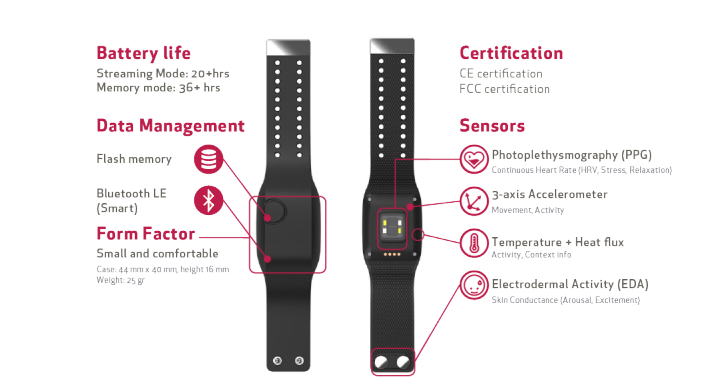
\includegraphics[width=\columnwidth]{images/Empatica.png}
	\caption{Empatica E4 features \parencite{emp}}
	\label{fig:empatica}
\end{figure}



\subsection*{Motion Capture}
The OptiTrack Motion Capture System is a motion capture system that uses an array of 12 high-speed cameras equipped with advanced optics and infrared sensors. These cameras are positioned to cover a designated area, creating a three-dimensional space where every movement is tracked and recorded. The system detects reflective markers placed on key points of a subject's body. As the subject moves within the camera's field of view, the system tracks the spatial position and orientation of these markers, seamlessly translating physical movements into digital data. 

For tracking the human body, the system uses a set of 25 marker points, which are placed at strategic points as shown in {\autoref{fig:opti3}}. This configuration ensures a thorough capture of the upper body movements. The calibration process is a critical step where each marker on the subject's body is meticulously mapped onto a digital skeleton model. This mapping ensures that the system can accurately track the movements of each marker in relation to the body's overall structure.The system individually tracks each marker as the subject moves, allowing for a detailed representation of motion.
The Motive software, integral to the OptiTrack system, plays a key role here. It enables users not only to visualize the movements in real time but also to record and analyze the data. The software translates the positional data of the markers into a skeletal animation, offering a clear and dynamic representation of the subject's movements.

\begin{figure}[h]
    \centering
    % First image
    \begin{subfigure}[b]{0.45\columnwidth}
        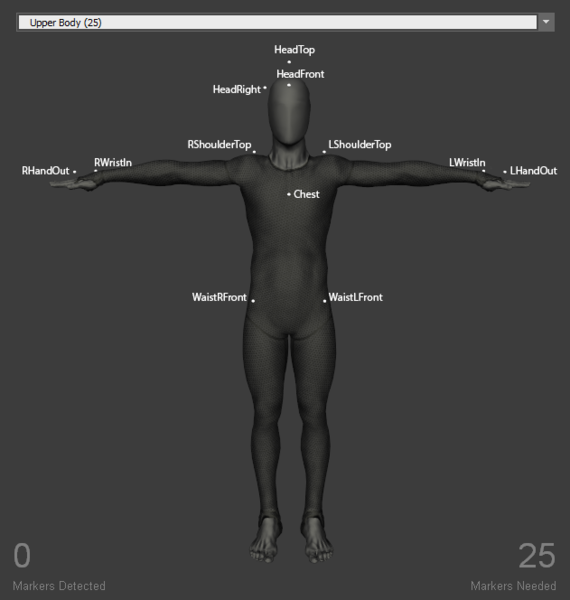
\includegraphics[width=\textwidth]{images/skleton.png}
        \caption{Front View }
        \label{fig:opti1}
    \end{subfigure}
    % Second image
    \begin{subfigure}[b]{0.45\columnwidth}
        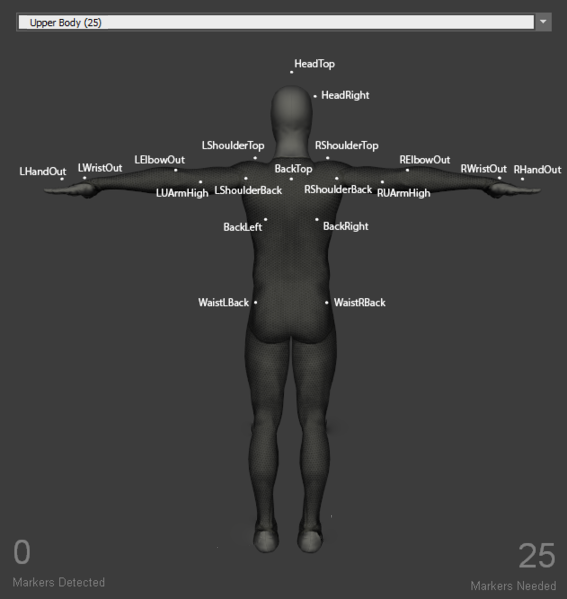
\includegraphics[width=\textwidth]{images/skeleton2.png}
        \caption{Back View }
        \label{fig:opti2}
    \end{subfigure}
    \caption{25 Upper Body Marker Set}
    \label{fig:opti3}
\end{figure}



\subsection{Photoplethysmogram-PPG}
\label{subsec:PPGtheory}

Photoplethysmogram (PPG) also known as  Blood Volume Pulse (BVP) are non-invasive optical techniques used to monitor changes in blood volume. They rely on the principles of light absorption and reflection to capture valuable information about cardiovascular activity. PPG and BVP sensors commonly found in wearable devices obtain PPG signals by transmitting light into the skin and measuring the amount of light either transmitted through or reflected back.\parencite{ppg} 

When the heart beats, it propels blood through the circulatory system, causing periodic changes in the volume of blood vessels. PPG sensors emit light into the tissue and measure the amount of light that is either absorbed or reflected back. During each heartbeat, blood absorbs more light, leading to a decrease in the amount of light detected by the sensor. Between heartbeats, when blood flow is less pulsatile, more light is detected.\parencite{ppg2}

The resulting waveforms from PPG typically consist of a series of peaks and troughs, with each peak corresponding to a heartbeat (systole) and each trough representing the resting period between beats (diastole). By analyzing the time intervals between these peaks, the heart rate can be calculated. This heart rate measurement is fundamental and provides valuable information about a person's cardiovascular health and overall fitness level. It serves as a key metric in various applications, including exercise tracking, medical diagnosis and in our case here stress assessment.

Furthermore, PPG signals enable the assessment of heart rate variability (HRV). HRV is the variation in time between successive heartbeats and is an essential indicator of the autonomic nervous system's activity. By analyzing the subtle changes in the intervals between PPG peaks, HRV can be quantified. High HRV typically indicates a healthy heart and a well-balanced autonomic nervous system, while reduced HRV can be associated with stress, illness, or various medical conditions. HRV analysis provides insights into the body's ability to adapt to different situations and is valuable for assessing stress levels, mental well-being, and overall cardiovascular health.

Other measures that can be derived from PPG data include  and estimation of blood oxygen saturation levels (SpO2), valuable for respiratory and circulatory health assessment. PPG can also be used to estimate respiration rate, reveal vasomotor activity changes associated with the autonomic nervous system, emotions, or vascular health, and provide insights into arterial stiffness and blood flow dynamics as well as blood pressure. First derivative and second derivates of PPG signals can also be analyzed. The first derivative (Velocity Plethysmogram, VPG) and the second derivative (Acceleration Plethysmogram, APG) features can be used for  blood pressure estimation etc.\parencite{apg}


\begin{figure}[h]
    \centering
    % First image
    \begin{subfigure}[b]{0.55\columnwidth}
        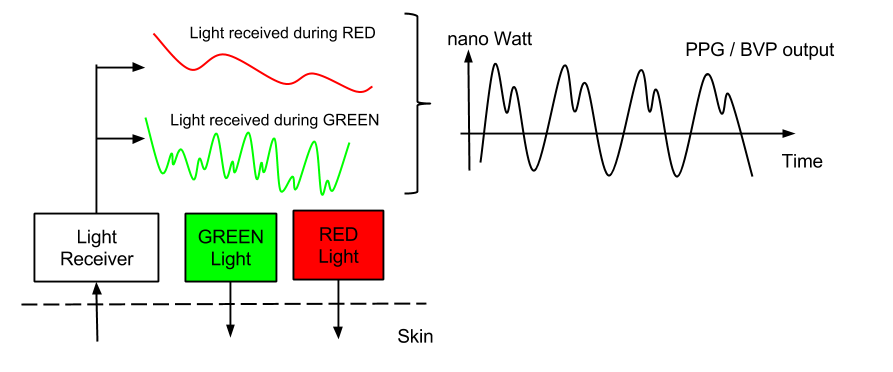
\includegraphics[width=\textwidth]{images/PPG.png}
        \caption{PPG process}
        \label{fig:ppg}
    \end{subfigure}
    % Second image
    \begin{subfigure}[b]{0.35\columnwidth}
        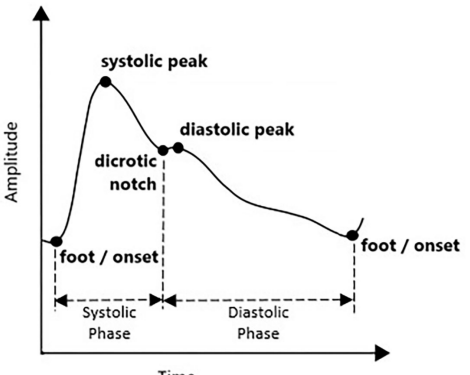
\includegraphics[width=\textwidth]{images/ppg2.png}
        \caption{Typical PPG Waveform}
        \label{fig:phone2}
    \end{subfigure}
    \caption{\parencite{emp} \parencite{apg}}
    \label{fig:phone}
\end{figure}



\subsection{Electrodermal Activity-EDA}
\label{subsec:EDAtheory}

Electrodermal Activity (EDA), also known as the galvanic skin response(GSR), is a way to measure changes in how our skin conducts electricity. Even moderate amounts of sweating that are not observable at the skin surface can alter skin electrical conductivity. The more the body sweats, the more conductive the skin becomes, and this change can be measured to infer physiological or psychological states.More specifically  EDA measures the skin's electrical conductance changes, which depend on the quantity of sweat secreted by eccrine sweat glands in the hypodermis of the palmar and plantar regions. Sweat secreted in the palmar and plantar regions is caused mainly by central nervous activity related to affective and cognitive states, including mental or emotional sweating. Thus EDA becomes one of the promising noninvasive methods widely used in detecting stress and emotion. EDA is a powerful method for real-time measurement and could be used as an index of emotional or cognitive stimulation related to stress.\parencite{gellman2020behavioral}.EDA is useful in several ways: it shows how we respond emotionally, helps us see how our body reacts to stress etc. It acts as a biomarker for emotional responsiveness and serves as a key indicator for stress-related bodily responses. 

Electrodermal Activity (EDA) comprises two main components: the tonic and phasic components. The tonic component, also known as skin conductance level (SCL), reflects slow and consistent changes in the signal's background. In contrast, the phasic components, referred to as skin conductance response (SCR) or spontaneous fluctuation of skin response, are the rapid and momentary fluctuations within the signal that occur within specific time intervals \parencite*{hernando2017feature}. SCR appears in response to stimuli activating the sympathetic nervous system. Consequently, SCR can be linked to a stimulus and can be valuable in measuring cognitive stress levels. However, directly extracting the components of EDA isn't straightforward.

When EDA sensors measure skin conductivity (SC) signals, they typically yield results in microsiemens. To extract the SCL and SCR components accurately, it is necessary to deconvolve the SC signals \parencite[postnote]{alexander2005separating}. Without proper separation of the original SC signals, overlapping SCRs can lead to less precise information during feature extraction . Therefore, it is crucial to perform deconvolution to distinguish the SCR and SCL signals effectively.

\begin{figure}[hb]
	\centering
	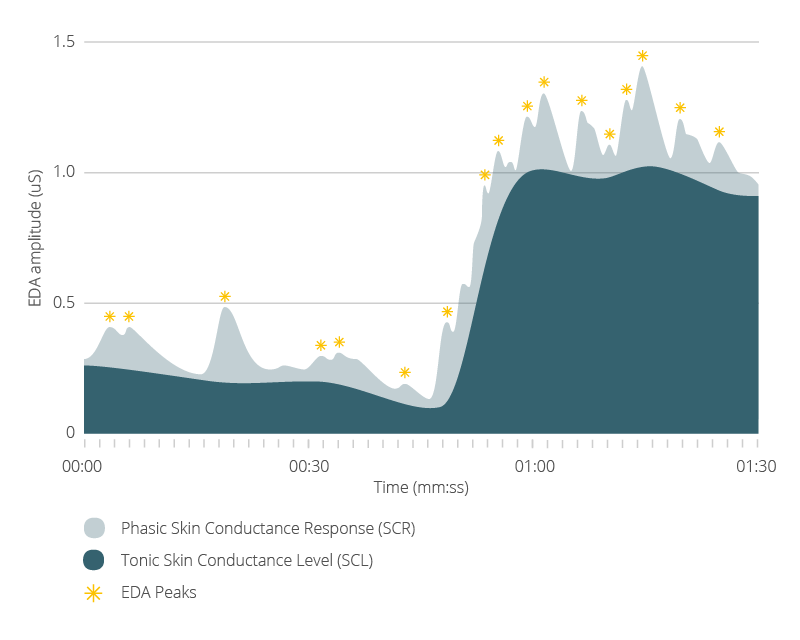
\includegraphics[width=\columnwidth]{images/EDA-example-graph.png}
	\caption{EDA Example signal - \parencite{eda}}
	\label{fig:eda sig}
\end{figure}



\section{UR10 robot and Collsion Avoidance }

\section{Stress Classification}


